%%%%%%%% ICML 2023 EXAMPLE LATEX SUBMISSION FILE %%%%%%%%%%%%%%%%%

\documentclass{article}

% Recommended, but optional, packages for figures and better typesetting:
\usepackage{microtype}
\usepackage{graphicx}
\usepackage{subfigure}
\usepackage{booktabs} % for professional tables

% hyperref makes hyperlinks in the resulting PDF.
% If your build breaks (sometimes temporarily if a hyperlink spans a page)
% please comment out the following usepackage line and replace
% \usepackage{icml2023} with \usepackage[nohyperref]{icml2023} above.
\usepackage{hyperref}


% Attempt to make hyperref and algorithmic work together better:
\newcommand{\theHalgorithm}{\arabic{algorithm}}

% Use the following line for the initial blind version submitted for review:
\usepackage[accepted]{icml2023}
% If accepted, instead use the following line for the camera-ready submission:
% \usepackage[accepted]{icml2023}

% For theorems and such
\usepackage{amsmath}
\usepackage{amssymb}
\usepackage{mathtools}
\usepackage{amsthm}
\usepackage{multirow}
% if you use cleveref..
\usepackage[capitalize,noabbrev, nameinlink]{cleveref}

%%%%%%%%%%%%%%%%%%%%%%%%%%%%%%%%
% THEOREMS
%%%%%%%%%%%%%%%%%%%%%%%%%%%%%%%%
\theoremstyle{plain}
\newtheorem{theorem}{Theorem}[section]
\newtheorem{proposition}[theorem]{Proposition}
\newtheorem{lemma}[theorem]{Lemma}
\newtheorem{corollary}[theorem]{Corollary}
\theoremstyle{definition}
\newtheorem{definition}[theorem]{Definition}
\newtheorem{assumption}[theorem]{Assumption}
\theoremstyle{remark}
\newtheorem{remark}[theorem]{Remark}

% Todonotes is useful during development; simply uncomment the next line
%    and comment out the line below the next line to turn off comments
%\usepackage[disable,textsize=tiny]{todonotes}
\usepackage[textsize=tiny]{todonotes}


% The \icmltitle you define below is probably too long as a header.
% Therefore, a short form for the running title is supplied here:
\icmltitlerunning{DRL for Energy Management}

\begin{document}

\twocolumn[
\icmltitle{Deep Reinforcement Learning for Energy Management in Residential Housing}

% It is OKAY to include author information, even for blind
% submissions: the style file will automatically remove it for you
% unless you've provided the [accepted] option to the icml2023
% package.

% List of affiliations: The first argument should be a (short)
% identifier you will use later to specify author affiliations
% Academic affiliations should list Department, University, City, Region, Country
% Industry affiliations should list Company, City, Region, Country

% You can specify symbols, otherwise they are numbered in order.
% Ideally, you should not use this facility. Affiliations will be numbered
% in order of appearance and this is the preferred way.
\icmlsetsymbol{equal}{*}

\begin{icmlauthorlist}
    \icmlauthor{Tim Walter}{yyy}
\end{icmlauthorlist}

\icmlaffiliation{yyy}{Department of Scientific Computing, Technical University of Munich, Munich, Germany}


\icmlcorrespondingauthor{Tim Walter}{tim.walter@tum.de}


% You may provide any keywords that you
% find helpful for describing your paper; these are used to populate
% the "keywords" metadata in the PDF but will not be shown in the document
\icmlkeywords{Machine Learning, ICML}

\vskip 0.3in
]

% this must go after the closing bracket ] following \twocolumn[ ...

% This command actually creates the footnote in the first column
% listing the affiliations and the copyright notice.
% The command takes one argument, which is text to display at the start of the footnote.
% The \icmlEqualContribution command is standard text for equal contribution.
% Remove it (just {}) if you do not need this facility.

%\printAffiliationsAndNotice{}  % leave blank if no need to mention equal contribution
\printAffiliationsAndNotice % otherwise use the standard text.

\begin{abstract}
    This paper provides a novel formulation of the carbon emission minimization problem within a smart home. The environment includes an energy storage system, a heat pump, and a flexible demand. The environment is formulated as a Markov Decision Process and tested using state of the art reinforcement learning methods. The effectiveness of the algorithms is compared to rule-based controllers. In addition, three variations of the environment are explored in an effort to improve the formulation in terms of learnability.
\end{abstract}

\section{Introduction}\label{sec:introduction}
The operations of buildings account for 30\% of global final energy consumption and 26 \%
of global energy-related greenhouse-gas emissions \cite{IEA.06.01.2024}. This makes the optimization of energy consumption a major concern for environmental sustainability. This paper investigates the application of Deep Reinforcement Learning (DRL) to streamline energy usage within a single-family home, leveraging solar panels, electric batteries, heat pumps, and flexible demand mechanisms. The primary aim is to reduce the carbon footprint associated with housing operations.

\section{Related Work}\label{sec:related_work}
The application field of smart energy management encompasses a wide range of problems, such as heating  and cooling \cite{Blum.2021}\cite{ThomasSchreiber.2020}, flexible demand response \cite{Jin.2021} and energy storage \cite{Nakabi.2021}. Moreover, the scale and level of detail of the tackled problems vary greatly, going from single buildings \cite{Blum.2021}, to microgrids \cite{Nakabi.2021} \cite{Castellanos.04.12.2022} to eventually continent wide electricity grids \cite{Horsch.2018}. The two most promising approaches to solve such problems are classical Model Predictive Control (MPC) \cite{Basantes.2023} and Reinforcement Learning (RL) \cite{Nakabi.2021} \cite{Jin.2021} \cite{ThomasSchreiber.2020}\cite{Zhu.2022}. Furthermore, there are also hybrid approaches that combine the two methods \cite{JavierArroyo.2022}.
\\~\\
This paper is mainly inspired by \cite{Nakabi.2021}, who describe a microgrid environment with generation, storage and consumers and optimized electricity pricing
using various deep reinforcement learning algorithms.

\section{Environment}\label{sec:environment}
The main contribution of this work is an environment modeling a single-family household, consisting of a Rooftop Solar Array (RSA), an Energy Storage System (ESS), a Thermostatically Controlled Load (TCL), and a Flexible Demand Response (FDR). The environment is a mixture of replayed data and dynamic components. It is built on the Gymnasium framework \cite{Towers.2023} and available on GitHub\footnote{https://github.com/TimWalter/smart-energy-controller}. The main objective is minimizing the CO2eq emissions. The task is split into week-long episodes with hourly resolution, to capture daily and weekly patterns of demand and generation.
\par
The RL paradigm requires the formulation as a Markov Decision Process, consisting of a transition function, action and observation spaces, and a reward function. The transition function is given by the replayed data and the dynamics of the components in the following. The observation space is a bounded subset of $\mathbb{R}^{11+H}$, with the observables given in \cref{tab:observation_space}. The action space is summarized in  \cref{tab:action_space}. The reward function is described in \cref{ssec:reward_function}.

\subsection{Replayed Data}\label{ssec:static_components}
The data was either initially given in hourly resolution or down-sampled by averaging. The most relevant observables are displayed exemplary in \cref{fig:static_components}.
\par
The auxiliary information included weather and time data, which provided means for the agent to predict the carbon intensity of the electricity mix and the heating demand. It was sourced from the Photovoltaic Geographical Information System (PVGIS) \cite{ThomasHuld.2012}.
\par
The RSA was simulated using the PVLIB library \cite{F.Holmgren.2018}, with panel specifications from the CEC database \cite{Dobos.2012}\cite{Boyson.2007}.
\par
The household's energy demand was sourced from the UCI archive \cite{GeorgesHebrail.2006}. Since the consumption was unraveled for different rooms, the kitchen, electric water heater and air conditioner were modeled as inflexible demand, while the laundry room as flexible demand.
\par
The direct carbon intensity of the electricity mix at any given time was sourced from Electricity Maps \cite{ElectricityMaps.2023}. 
\begin{figure}[H]
    \centering
    \setlength{\abovecaptionskip}{0pt}
    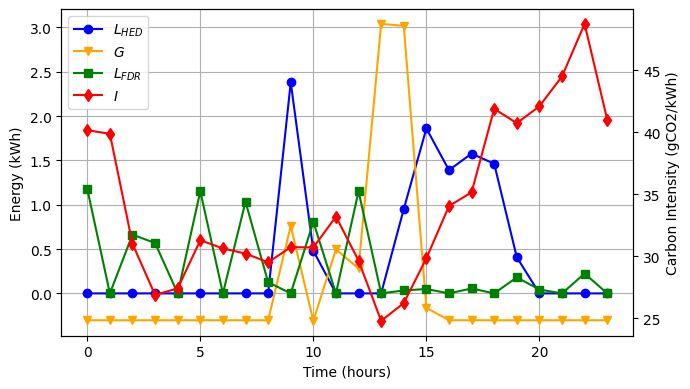
\includegraphics[width=0.45\textwidth]{figures/static_components.png}
    \caption{Replayed data for the first 24 hours.}
    \label{fig:static_components}
\end{figure}

\subsection{Energy Storage System}
The ESS is connected to the grid and the RSA. The charge is subject to the following dynamics
\begin{equation}
    B_t = \max\{0, B_{t-1} - D_s + C_t \sqrt{\nu} - \frac{D_t}{\sqrt{\nu}}\}.
\end{equation}
Here, $B_t \in [0, B_{max}]$ is the charge at time $t$ and $B_{max}$ is the capacity. Furthermore, $\nu$ denotes the round trip efficiency, $D_s$ the self-discharge rate, $C_t \in [0, C_{max}]$ the charge rate with maximum $C_{max}$, and $D_t \in [0, D_{max}]$ the discharge rate with its respective maximum $D_{max}$. 

\subsection{Flexible Demand Response}
The FDR can be influenced stochastically in a running time window of length $H$ by a signal $a_{fdr, t} \in [-1 , 1]^H$. Whether the power is consumed is determined by a Bernoulli process, with probabilities
\begin{equation}
    p_t = \text{clip}\left(s + a_{fdr, t} * \exp\left(\frac{-1}{\beta}\left|t - t_{s}\right|\right), 0, 1\right),
\end{equation}
where $s \in \{0,1\}^{H}$ indicates the desired consumption with elements $s_i = \begin{cases}
    1 & \text{if } t_i \leq t \\
    0 & \text{else}
\end{cases}$, $\beta$ is a patience parameter, and $t_{s} \in \mathbb{R}^{H}$ is the desired consumption time. If consumption is delayed more than once, $\frac{2}{H-1}$ of the power is consumed in each time step to ensure that all power has been consumed after the time window. This aims to facilitate learning by preventing infinite delays or a large correction at episode termination.

\subsection{Thermostatically Controlled Load}\label{ssec:tcl}
The TCL encapsulates all devices that aim to maintain the temperature of a given heat mass. To utilize such loads as energy storage, the temperature of the heat mass is allowed to fluctuate within a given range. The TCL is modeled as a second-order system \cite{Sonderegger.1978} with the following dynamics:
\begin{equation}
    \begin{split}
        T_t &= T_{t-1} + \frac{1}{r_a} (T_{a, t} - T_{t-1}) \\
        &+ \frac{1}{r_b} (T_{b,t} - T_{t-1}) \\
        &+ \frac{1}{r_h} L_{TCL} a_{tcl,t} + q,
    \end{split}
\end{equation}
where $T_t$ is the indoor temperature at time $t$, $r_a$ is the thermal mass of the air, $T_{a, t}$ is the current outdoor temperature, $r_b$ is the thermal mass of the building material, and $T_{b, t}$ is the current building mass temperature, that evolves with
\begin{equation}
    T_{b, t} = T_{b, t-1} + \frac{1}{r_b} (T_{t-1} - T_{b, t-1}),
\end{equation}
$\frac{1}{r_h}$ is the power-to-heat coefficient, $L_{TCL}$ is the nominal power, 
$a_{tcl_t} \in [-1, 1]$ is the heating signal, and $q$ is the unintended heat drift. The heating signal is constrained by the desired temperature range, enforced through a backup controller as follows:
\begin{equation}
    a_{tcl, t} = \begin{cases}
        -1 & \text{if } T_t \geq T_{max} \\
        1 & \text{if } T_t \leq T_{min} \\
        a_{tcl, t} & \text{else,} 
    \end{cases}
\end{equation}
where $T_{max}$ and $T_{min}$ define the desired temperature range. 

\begin{table}
\caption{Observation Space.}
\label{tab:observation_space}
\vskip 0.15in
\begin{center}
\begin{small}
\begin{sc}
\begin{tabular}{lcr}
\toprule
Observable & Symbol & Replayed\\
\midrule
Carbon Intensity & $I$ & X\\
    Household Energy Demand & $L_{HED}$ & X\\
    Rooftop Solar Generation & $G$ & X\\
    ESS Charge & $B$ & \\
    FDR power in window & $L_{FDR}$ &\\
    Indoor temperature & $T$ & \\
    Time step & $t$ & X\\
    Month of Year & $MoY$ & X \\
    Solar Irradiation & $SI$ & X\\
    Solar Elevation & $SE$ & X\\
    Outdoor temperature & $T_a$ & X \\
    Wind Speed & $WS$ & X\\
\bottomrule
\end{tabular}
\end{sc}
\end{small}
\end{center}
\vskip -0.1in
\end{table}

\begin{table}
\caption{Action Space.}
\label{tab:action_space}
\vskip 0.15in
\begin{center}
\begin{small}
\begin{sc}
\begin{tabular}{lcr}
\toprule
Action & Min. Meaning & Max. Meaning\\
\midrule
$a_{ess}$ & Discharge & Charge \\ 
    $a_{fdr}$ & Delay     & Expedite \\
    $a_{tcl}$ & Cooling   & Heating\\
\bottomrule
\end{tabular}
\end{sc}
\end{small}
\end{center}
\vskip -0.1in
\end{table}

\subsection{Reward Function} \label{ssec:reward_function}
CO2eq emissions are modeled naively as carbon intensity $I_t$ times produced energy $E_p$ minus consumed energy $E_c$. The given objective is augmented by a temperature discomfort penalty $DC$ to bias towards the desired temperature. 
The resulting reward function is
\begin{flalign}
    r_t &= I_t (E_p - E_c) - DC && \\
    \begin{split}
        E_c &= L_t + \frac{1}{r_h} L_{TCL} a_{tcl,t} + C_t \\
        &+ \sum_{p \in U_e} p_r + \sum_{p \in U_d} \frac{2p}{H-1}
    \end{split} && \\
    E_p &= G_t + D_t  && \\
    DC &= \delta \exp(|T_t - \frac{T_{max} + T_{min}}{2}), &&
\end{flalign}
where $U_e$ is the set of consumed FDR, $p_r$ is the remaining power after discounting, $U_d$ is the set of delayed FDR, and $\delta$ the discomfort coefficient. 
\par
Given that the task formulation is episodic, it differs from the real-world problem which has an infinite horizon. In the real-world problem, the initial state of the upcoming week is influenced by the past week. Therefore, to accurately reflect this, a correction is required at termination to evaluate the remaining state. The terminal reward is corrected by
\begin{flalign}
    reward &\mathrel{+}= I_t B_t && \\
    reward &\mathrel{+}= I_t (- \sum_{p \in U} p_r) && \\
    reward &\mathrel{+}= I_t (- r_h\left|T_t - \frac{T_{max}+T_{min}}{2}\right|) && 
\end{flalign}
where $U$ is the set of remaining FDR.

\section{Experiments}\label{sec:limitations}
\begin{table*}[t]
\label{tab:experiments}
\caption{Accumulated rewards split by origin per experiment. Evaluation were done after every epoch and the best result is shown.}
\vskip 0.15in
\begin{center}
\begin{small}
\begin{sc}
\begin{tabular}{lcccccr}
\toprule
Experiment & Algorithm & ESS & FDR & TCL & Discomfort & Total \\
\midrule
\multirow{4}{*}{Full Environment} 
    & Idle      & 0.00   & -3173.56 & \textbf{-9887.61}  & -5912.63 & -18973.80 \\
    & Threshold & \textbf{633.24} & \textbf{-3071.35} & -9957.07  & -5557.23 & -17952.41 \\
    & PPO       & 0.00   & -3233.98 & -10825.89 & \textbf{-788.15} & \textbf{-14847.02} \\
    & SAC       & 60.24  & -3087.39 & -14692.60 & -1637.00 & -19356.75 \\
\midrule
\multirow{4}{*}{Hypothesis 1}
    & Idle      & 0.00   & -3173.56 & \textbf{-9887.61} & -5912.63 & -18973.80 \\
    & Threshold & \textbf{633.24} & \textbf{-3068.56} & -9957.07 & -5557.23 & -17949.62 \\
    & PPO       & 0.00   & -3151.34 & -11058.75& \textbf{-531.89} & \textbf{-14741.98} \\
    & SAC       & -40.18 & -3192.11 & -14329.95 & -1258.60 & -19820.84 \\
\midrule
\multirow{4}{*}{Hypothesis 2} 
    & Idle      & 0.00   & -3173.56 & \textbf{-9887.61} & -5912.63 & -18973.80 \\
    & Threshold & \textbf{633.24} & -3068.56 & -9957.07 & -5557.23 & -17949.62 \\
    & PPO       & 488.58 & -3035.30 & -10755.65 & \textbf{-3152.03} & \textbf{-14454.40} \\
    & SAC       & 157.94 & \textbf{-2969.78} & -10114.51 & -4906.66 & -17832.01 \\
\midrule
\multirow{4}{*}{Hypothesis 3} 
    & Idle      & 0.00   & -3173.56 & \textbf{-9887.61} & -5912.63 & -18973.80 \\
    & Threshold & 633.24 & -3068.56 & -9957.07 & \textbf{-5557.23} & \textbf{-17949.62} \\
    & PPO       & \textbf{650.49} & -3170.04 & -10512.15 & -5913.87 & -18945.57 \\
    & SAC       & 599.65 & \textbf{-2969.36} & -52971.76 & -13164.96 & -67506.43 \\
\bottomrule
\end{tabular}
\end{sc}
\end{small}
\end{center}
\vskip -0.1in
\end{table*}

As non-learning baselines an idle policy, which would always return zero actions, whose cumulative reward in the first episode is shown in \cref{fig:reward_idle}, and a thresholding policy, see \cref{sec:thresholding_baseline}, were implemented.

\begin{figure}[H]
    \centering
    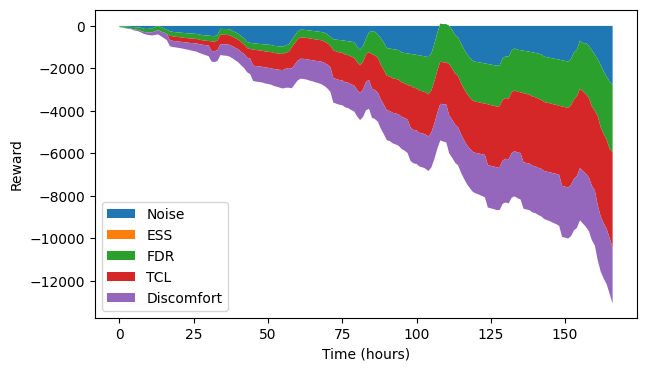
\includegraphics[width=0.45\textwidth]{figures/idle_reward.png}
    \caption{Cumulative reward for the idle policy.}
    \label{fig:reward_idle}
\end{figure}

As learning agents, Soft Actor Critic (SAC) \cite{Haarnoja.04.01.2018} and Proximal Policy Optimization (PPO) \cite{Schulman.20.07.2017} were chosen. Both implementations were taken from stable baselines 3 \cite{AntoninRaffin.2021}, for details see \cref{sec:sac} and \cref{sec:ppo}.
\par
To allow for differentiation on which sub-tasks the agent performs well, the reward was split by the component of origin, as in \cref{sec:split_reward}. 
\par
The results of all experiments are shown in \cref{tab:experiments}. Since the initial task did not yield reward convergence surpassing the baselines, as shown in \cref{fig:training_curve}, three hypothesis with accompanying modifications to the environment were tested. The changes were cumulative and further details can be found in \cref{sec:training_procedure}.
\begin{figure}[H]
    \centering
    \setlength{\abovecaptionskip}{0pt}
    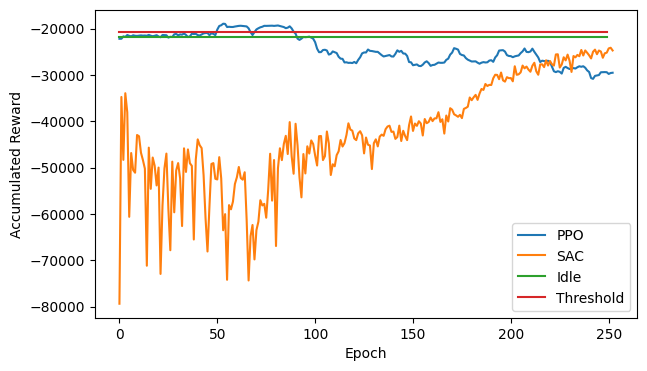
\includegraphics[width=0.45\textwidth]{figures/training_curve.png}
    \caption{Training curve of the Full Environment.}
    \label{fig:training_curve}
\end{figure}


\subsection{Scheduling, Stochasticity, and Dimensionality}
The challenge of learning in the FDR sub-task is innate in scheduling \cite{Zhang.23.10.2020} but is further complicated by the stochastic control. Furthermore, it bloats the dimensionality of the spaces with decreasing resolution, since the time window was always 24 hours.
\par
To ease those challenges the control was changed to deterministic, and scalar and the observation included only the sum of the time window. These changes are equivalent to the assumption that the optimal policy is invariant to $U_e$ as long as the sum is maintained and that $\beta = \infty$.
\par
The modified task only showed improvements for minutely resolution, which suggests that high dimensionality is a problem. However, since convergence was still absent, the inefficiency of the other changes could not be concluded.


\subsection{Hard Exploration}
The environment still provides a vast exploration space, due to the continuity of the spaces and the length of the episodes. Moreover, there is significant noise from the RSA and fixed demand on the reward. Moreover, a lot of observables are only relevant for estimating the future carbon intensity. 
\par
To address this the minutely resolution was omitted, the action space for PPO was discretised, the fixed demand and RSA were removed from the observables and reward calculation, and the agents were trained separately for every sub-task. Lastly, the replay buffer for SAC was initialized with transitions of the threshold algorithm, providing a warm start \cite{Wang.20.06.2023}.
\par
The result indicated, that the discretisation aided PPO in learning the ESS but hindered in the TCL sub-task, hinting too coarse discretisation. SAC did not benefit from the warm start after a few epochs. 


\subsection{Delayed or Deceptive reward}
Another challenge of the setting is the reward structure for charging the ESS, expediting the FDR and heating or cooling the TCL. The rewards of those actions always occur delayed and only if the respective counter action is performed at a higher carbon intensity, which can be problematic \cite{Sutton.1984}. Moreover, the rewards might even be deceptive, since those actions are necessary for an effective policy but only ever receive negative reward.
\par
To test the hypothesis, the reward was transferred to an accumulating observable and only actuated in the terminal state, which should encourage the agent to evaluate the entire trajectory of an episode holistically.
\par 
Since the task was hardened by this change performance was expectedly decreased for TCL and FDR. However, the ESS sub-task showed signs of improvements but no convergence within the 250 epochs.

\section{Discussion}\label{sec:discussion}
This paper provides an open challenge with a novel formulation of the problem of carbon intensity minimization in a smart home environment. Various experiments were run to test hypothesis on the cause of the learning inefficiency. While no single hypothesis led to a complete solution, two out of three aided the learning of some sub-tasks. A promising future direction would be to combine the various policies into an ensemble, with each controlling one subsystem. 


\bibliography{literature.bib}
\bibliographystyle{icml2023}


%%%%%%%%%%%%%%%%%%%%%%%%%%%%%%%%%%%%%%%%%%%%%%%%%%%%%%%%%%%%%%%%%%%%%%%%%%%%%%%
%%%%%%%%%%%%%%%%%%%%%%%%%%%%%%%%%%%%%%%%%%%%%%%%%%%%%%%%%%%%%%%%%%%%%%%%%%%%%%%
% APPENDIX
%%%%%%%%%%%%%%%%%%%%%%%%%%%%%%%%%%%%%%%%%%%%%%%%%%%%%%%%%%%%%%%%%%%%%%%%%%%%%%%
%%%%%%%%%%%%%%%%%%%%%%%%%%%%%%%%%%%%%%%%%%%%%%%%%%%%%%%%%%%%%%%%%%%%%%%%%%%%%%%
\newpage
\appendix
\onecolumn


\section{Further Environment Details} \label{sec:environment_details}
The replayed data was mainly recorded or simulated  in the time from 07.01.2007 to 28.12.2008. Although some episodes had to be left out due to missing data, there were more than 100 episodes, of which 95 were supposed to be used for training, 4 for testing and the rest for evaluation. The power was standardized to kilowatts, while the energy was simply kWmin or kWh depending on the resolution. However, es the time steps are equidistant, power and energy can be modeled equivalently, since the power was assumed to be constant over the time step. Only some constants had to be adapted. The location of the house was in France near Paris.
\par
The carbon intensity data was only available from 2021 and 2022 for France, so the carbon intensity might be biased, since the electricity mix might have drifted over the years. However, the daily, weekly and yearly frequencies should still be captured, although potentially drifted. The unit of carbon intensity is gram of CO\textsubscript{2} equivalent emissions per kWh or kWmin.
\par To prevent the ESS from overcharging or overdischarging, the rates were further constrained by the current charge and capacity, such that actually $C_t \in [0, \min\{C_{max}, \frac{B_{max} - B_t + D_s}{\sqrt{\nu}}\}]$ and $D_t \in [0, \min\{D_{max}, (B_t - D_S) \sqrt{\nu}\}]$.

\section{Thresholding Baseline} \label{sec:thresholding_baseline}
\begin{equation}
    a_t = \left\{
        \begin{array}{ll}
            \begin{bmatrix} \phantom{-}1 & [1]^H & \psi0.1 \end{bmatrix} & \text{if } I_t < \phi_1 \\
            \begin{bmatrix} -1 & [0]^H & \phantom{\psi}0\phantom{.1} \end{bmatrix} & \text{if } I_t > \phi_2 \\
            \begin{bmatrix} \phantom{-}0 & [0]^H & \psi0.1 \end{bmatrix} & \text{else}
        \end{array}
    \right.
\end{equation}
where $\phi_1$ and $\phi_2$ are the lower and upper threshold respectively, while $\psi = sign(T_t -\frac{T_{max} + T_{min}}{2})$.
The parameters for the thresholding algorithm were $\psi_1 = 65$ and $\psi_2 = 85$.

\section{SAC}\label{sec:sac}
SAC is a squashed Gaussian policy, that employs entropy regularization, which adds a bonus reward in each time step proportional to the current entropy of the policy in an aim to encourage exploration. Furthermore, two Q-functions are learned and their minimal estimate is used to update the policy. The objective function for SAC is:
\begin{equation}
    \max _\theta \underset{\substack{s \sim \mathcal{D} \\ \xi \sim \mathcal{N}}}{\mathbb{E}}\left[\min _{j=1,2} Q_{\phi_{\hat{j}}}\left(s, \tilde{a}_\theta(s, \xi)\right)-\alpha H(\pi_\theta \mid s)\right]
\end{equation}
where $\theta$ denotes the policy parameter, $\xi$ normal Gaussian noise, $\tilde{a}_\theta(s, \xi)$ the action sampled from the current policy, $\alpha$ the entropy regularization coefficient, and $H(\pi_\theta \mid s) = \log \pi_\theta\left(\tilde{a}_\theta(s, \xi) \mid s\right)$ the entropy of the policy. The action samples are obtained as $\tilde{a}_\theta(s, \xi) = tanh(\mu_\theta(s)+\sigma_\theta(s) \odot \xi)$


\section{PPO}\label{sec:ppo}
PPO is a trust-region based policy gradient method, which solves a constrained policy update policy via SGD. It achieves the trust region remarkably simple, by employing the following update objective:
\begin{flalign}
    \theta_{k+1} &= \arg \max _{\theta} \underset{\substack{s \sim \mathcal{D} \\ a \sim \pi_{\theta_k}}}{\mathbb{E}} \left[ L(s,a)\right]&& \\
    L(s,a)&=\min \left(\left|\frac{\pi_\theta(a \mid s)}{\pi_{\theta_k}(a \mid s)}\right|, 1\pm \epsilon \right) A^{\pi_{\theta_k}}(s, a)&&
\end{flalign}
where $A^{\pi_{\theta_k}}(s, a)$ is the advantage of the current policy, and $\epsilon$ the trust region hyperparameter, clipping the update size. Alternatively, PPO can also be implemented using a KL-divergence constraint.


\section{Training Procedure} \label{sec:training_procedure}

All experiments were run for 250 episodes and in hourly resolution. Due to the encountered difficulty all were replaying only a single episode. Furthermore, the initial conditions, the initial indoor temperature $T_0$, building mass temperature $T_{b,0}$, and initial charge $B_0$, were fixed. The training parameters are shown in \ref{tab:training_parameters}. 
\begin{table}[H]
\label{tab:training_parameters}
\caption{Training Parameters}
\vskip 0.15in
\begin{center}
\begin{small}
\begin{sc}
\begin{tabular}{lr}
\toprule
Parameter & Value\\
\midrule
$B_{max}$ & 13.5 \\
$C_{max}$ & 1 \\
$D_{max}$ & 1 \\
$\nu$ & 0.95 \\
$D_s$ & 0.01 \\
$B_0$ & 0 \\
$H$ & 25 \\
$\beta$ & 20 \\
$\delta$ & 5 \\
$T_{0}$ & 20 \\
$T_{b,0}$ & 20 \\
$r_{a}$ & 0.04 \\
$r_{b}$ & 0.1 \\
$r_{h}$ & 0.05 \\
$q$ & 0.05 \\
$L_{TCL}$ & 5 \\
$T_{max}$ & 23 \\
$T_{min}$ & 18 \\
\bottomrule
\end{tabular}
\end{sc}
\end{small}
\end{center}
\vskip -0.1in
\end{table}

\section{Split Reward}\label{sec:split_reward}
\begin{flalign}
    r_{noise} &= I_t (G_t - L_t) && \\
    r_{ESS} &= I_t (D_t - C_t) && \\
    r_{FDR} &= I_t (-\sum_{p \in U_e} p_r - \sum_{p \in U_d} \frac{2p}{H-1}) && \\
    r_{TCL} &= I_t (-\frac{1}{r_h} L_{TCL} a_{tcl,t}) && \\ 
    r_{discomfort} &=- \delta exp(|T_t - \frac{T_{max} + T_{min}}{2}) &&
\end{flalign}
The reward for TCL was split, since maintaining the temperature is a very different task than minimizing the energy consumption.
%%%%%%%%%%%%%%%%%%%%%%%%%%%%%%%%%%%%%%%%%%%%%%%%%%%%%%%%%%%%%%%%%%%%%%%%%%%%%%%
%%%%%%%%%%%%%%%%%%%%%%%%%%%%%%%%%%%%%%%%%%%%%%%%%%%%%%%%%%%%%%%%%%%%%%%%%%%%%%%


\end{document}


% This document was modified from the file originally made available by
% Pat Langley and Andrea Danyluk for ICML-2K. This version was created
% by Iain Murray in 2018, and modified by Alexandre Bouchard in
% 2019 and 2021 and by Csaba Szepesvari, Gang Niu and Sivan Sabato in 2022.
% Modified again in 2023 by Sivan Sabato and Jonathan Scarlett.
% Previous contributors include Dan Roy, Lise Getoor and Tobias
% Scheffer, which was slightly modified from the 2010 version by
% Thorsten Joachims & Johannes Fuernkranz, slightly modified from the
% 2009 version by Kiri Wagstaff and Sam Roweis's 2008 version, which is
% slightly modified from Prasad Tadepalli's 2007 version which is a
% lightly changed version of the previous year's version by Andrew
% Moore, which was in turn edited from those of Kristian Kersting and
% Codrina Lauth. Alex Smola contributed to the algorithmic style files.
